\documentclass[a4paper]{article}

\usepackage{fullpage}
\usepackage[english]{babel}
\usepackage[utf8]{inputenc}
\usepackage{amsmath}
\usepackage{graphicx}
\usepackage{float}
\usepackage[colorinlistoftodos]{todonotes}
\usepackage{multirow}
\usepackage{array}
\usepackage{url}
\usepackage[labelfont=bf]{caption}
\usepackage[labelsep=period]{caption}
\usepackage[toc,page]{appendix}

\usepackage{listings}
\usepackage{color}
 
\definecolor{codegreen}{rgb}{0,0.6,0}
\definecolor{codegray}{rgb}{0.5,0.5,0.5}
\definecolor{codepurple}{rgb}{0.48,0.37,0.64}
\definecolor{codedarkpurple}{rgb}{0.66,0.11,0.37}
\definecolor{backcolour}{rgb}{0.99,0.99,0.99}

\usepackage{mathtools}
 
\lstdefinestyle{mystyle}{
    backgroundcolor=\color{backcolour},   
    commentstyle=\color{codegreen},
    keywordstyle=\color{codedarkpurple},
    numberstyle=\tiny\color{codegray},
    stringstyle=\color{codepurple},
    basicstyle=\footnotesize,
    breakatwhitespace=false,         
    breaklines=true,                 
    captionpos=b,                    
    keepspaces=true,                 
    numbers=left,                    
    numbersep=5pt,                  
    showspaces=false,                
    showstringspaces=false,
    showtabs=false,                  
    tabsize=2
}
 
\lstset{style=mystyle}

\title{% 
On the Difficulties Behind Automated Test Case Generation 
}

\author{%
\small Valentine Mairet \\
\texttt{4141784}
\and
\small Martin Rogalla \\
\texttt{4173635}
\and
\small Aleksandra Taneva \\
\texttt{4510488}
}

\begin{document}
\maketitle

\vfill 

\begin{abstract}
\noindent
Automated test case generation was introduced to make the life of software testers easier. 
However, some problems regarding the generation of test cases still remain. 
In this report, the EvoSuite tool for automated Java JUnit test case generation is run on 12 different Java classes to investigate the difficulties behind this automated process. 
Each class is chosen for its size, complexity, and how difficult it seems to test at first glance.
Additionally, this report provides an appendix with a short piece on the usability of EvoSuite and snippets of classes EvoSuite was run on. 
By correlating cyclomatic complexity with branch coverage, and with test readability, the hope is to find a reason behind the difficulty to test a specific branch, and to generate readable tests to help the developer generate oracles easier. 
The correlation coefficients found were insignificant, with 0.1753 and 0.3044 for cyclomatic complexity with branch coverage and with test readability respectively. 
Therefore, cyclomatic complexity does not have an influence on neither code coverage nor generated test readability.
However, it seems that the cause for low coverage lies deeper.
When tests require specific input that needs conscious intervention, EvoSuite does not seem to be able to generate such test. 
The tool cannot reason about the source code as a human would.
EvoSuite also fails at boundary testing. 
Moreover, when dealing with specific Java Generics input, EvoSuite cannot properly generate tests either. 
The results show that EvoSuite is highly optimized for branch coverage, but when it fails at doing so, the reason mostly lies within the reasoning needed to deal with the source code. 
\end{abstract}
\newpage

\tableofcontents
\newpage

\setlength{\parindent}{0cm}

\section{Introduction} 

Software testing is an essential component of software development that allows developers to assess the reliability and correctness of a software product.
Over the years, researchers have designed techniques to automatically produce test cases, where the code coverage criterion is the most commonly used guiding medium for the generation. 
Now, with the newest tools available, it has become possible to generate entire test suites with high coverage. 
One of these tools for Java software is the EvoSuite  framework \cite{FRASER2013}.

\subsection{EvoSuite} \label{evosuite}

EvoSuite is a tool that automatically generates JUnit tests with an evolutionary algorithm \cite{JUNIT,FRASER2013}. 
This tool can be directly run from the command line or through the Eclipse or IntelliJ IDEA IDEs, with the options to either generate tests according to the \textit{whole-test-suite} or \textit{single-target} approach \cite{FRASER2013}. 
It can also be configured to either generate tests class per class or for the entire project at once \cite{EVOSUITECLI}.

EvoSuite works at the bytecode level and collects all necessary information for test case generation from the bytecode via Java Reflection \cite{FRASER2013}. 
This means that EvoSuite can also be used for other programming languages that compile to Java bytecode (such as Scala or Groovy) \cite{VENNERS2008,SUBRAMANIAM2008}. 

There is, however, one problem associated with automatic test case generation, known as the \textit{oracle problem} \cite{BARR2015}. 
Automatic oracles that assert what the outcome of a test should be are possible when it comes to explicit events such as 'the program should not crash'. 
But when dealing with more complex outcomes, human intervention is necessary to specify oracles \cite{FRASER2013}. 
For this to be feasible, EvoSuite aims not only at high code coverage but also at small test suites that make manual oracle generation as easy as possible. 

\subsection{Limitations of EvoSuite}

But EvoSuite does not always get it right, and some coverage goals are occasionally not fulfilled \cite{FRASER2013}. 
This can be explained by a few language-related problems that are encountered by the EvoSuite tool during test case generation.

In particular, classes using Java Generics are problematic, as type erasure removes much of the useful information during compilation and all generic parameters are considered as Object. 
To overcome this problem, EvoSuite always inserts an Integer object into container classes, in order to cast returned Object instances back to Integer \cite{FRASER2013}. 
However, for a method with Generic input that is not compatible with an Integer object, things can go wrong. 

Additionally, other factors may contribute to explaining why EvoSuite does not always get it right.
There may be methods with inputs for which conscious human intervention is necessary, and there is no way for EvoSuite to know what the input is supposed to be \cite{FRASER2013}. 
An instance of this problem is a method that takes an integer and returns \textit{true} if that integer is prime. For a test to cover the \textit{true} branch and check the correctness of the code, the input must be a prime number. 

\subsection{This Research}

This paper poses the question of difficulty behind automated test case generation with EvoSuite and dives into the reasons why such difficulty exists. 
Why are certain pieces of code hard to generate tests for? 
Does EvoSuite fail at generating tests because the code is bad or too complex?
Does EvoSuite always generate readable tests to ease the generation of oracles by developers?

After a recap of previous work done on and with EvoSuite in section \ref{work}, the methods for this research are explained in detail in section \ref{methods}.
Then, the results are presented in section \ref{results}.
Lastly, this paper concludes the research executed and brings up a discussion on the implication of the results found. 

On a side note, an analysis of the usability of the EvoSuite tool is given. 
This analysis provides a few details on the problems encountered when using EvoSuite and what difficulties regarding the usage of the framework possibly hindered the progress of this research. 


\section{Previous Work} \label{work}

Previous work on and with EvoSuite has been done to prove automated test case generation could result in test suites with high code coverage and little test cases \cite{FRASER2013}.
The same team who presented EvoSuite additionally inquired upon the effectiveness of EvoSuite and the \textit{whole-test-suite} approach \cite{FRASER2014}. 

\subsection{Making of EvoSuite}

Making EvoSuite with the \textit{whole-test-suite} approach aimed at high code coverage and the generation of smaller test suites to make the specification of assertions as easy as possible \cite{FRASER2013}.

EvoSuite achieves this by selecting branch coverage as a coverage criterion and executing a genetic algorithm that selects a random population of test suites and evolves this population.
It stops the evolution process when a solution is found which fulfills the coverage criterion or when the set of resources (such as time or number of fitness evaluations) have been used up \cite{FRASER2013}. 

A solution is defined as a \textit{test suite}, which is represented as a set of test cases. 
A test case is represented by a sequence of statements. 
The fitness function estimates how close a solution is to covering \textit{all} branches by taking into account \textit{branch distance} for each branch, and the number of branches left to cover. 
It also takes into account the size of the solution, to make sure the generated test suite does not grow to large. 

It was shown that this approach fulfilled large coverage goals and succeeded at generating small enough test suites for easy oracle generation \cite{FRASER2013}. 
But what about the performance of the \textit{whole-test-suite} approach compared to \textit{single-target}?

\subsection{Whole Test Suite vs Single Target}

By comparing the coverage achieved by the \textit{whole-test-suite} and \textit{single-target} approach, it was establish that, in general, the \textit{whole} approach performs better \cite{FRASER2014,FRASER2015}.

Existing research has shown that the \textit{whole-test-suite} approach lead to better coverage results than the traditional \textit{single-target} approach. 
There was reasonable doubt on whether this would be the case when targeting difficult goals. 
An in-depth analysis was performed to study if this doubt could be confirmed in practice \cite{FRASER2014}.

EvoSuite was run on 100 different Java classes respectively for both techniques. 
It was found that indeed, the Whole approach had more difficulties when targeting difficult goals. 
However, these cases are very few compared to the cases for which Whole performed significantly better.
This thus confirmed that overall, \textit{whole-test-suite} is better. 





\section{Methods} \label{methods}

For automated test case generation to be optimal, the test suite needs to achieve high coverage while remaining relatively small for oracle generation \cite{FRASER2013}.
But remaining small does not necessary mean the generated test cases are readable for developers.
The target of our research is the difficulties regarding automated test case generation when using EvoSuite. 
Hence, this paper focuses mainly on the difficulty to achieve certain coverage goals and difficulty to generate readable tests. 
The two questions that arise from this focus are: what is the reason behind unfulfilled coverage goals and what can make EvoSuite generate illegible tests?

\subsection{Experiment}

In an attempt to provide answers, we execute an experiment, running the EvoSuite tool on 12 Java classes, each picked out of different projects, from open source software to our own. 
These classes were chosen according to size and complexity, and our own opinion on the difficulty to test such class. 
We estimated this difficulty based on whether a test would need a highly specific input to cover certain branches. 
We also designed or modified a few classes especially for this experiment.
The chosen classes are reported in Table \ref{classes}. 

{\setlength{\extrarowheight}{1ex}
\begin{table}[tbp]
\begin{center}
\small
\begin{tabular}{ m{7cm} p{2.5cm} p{2cm} }
\hline 
Class & Project & Source \\ [0.5ex]
\hline
PrimeChecker & EvoTest & Own \\ [0.5ex] 
IntStack & EvoTest & Own \\ [0.5ex]
EnglishNumberToWords & NumberToWords & Real's HowTo  \\ [0.5ex]
ColourPicker & EvoTest & Own \\ [0.5ex]
org.joda.time.chrono.ISOChronology & Joda-Time & GitHub \\ [0.5ex]
org.joda.time.DateTimeUtils & Joda-Time & GitHub \\ [0.5ex]
com.google.common.base.Optional & Guava & GitHub \\ [0.5ex]
com.google.common.base.Strings & Guava & GitHub \\ [0.5ex]
com.google.common.math.IntMath  & Guava & GitHub \\ [0.5ex]
com.google.common.graph.ImmutableGraph  & Guava & GitHub\\ [0.5ex]
\hline
\end{tabular}
\end{center}
\caption{For each class, the table reports which project the class belongs to, and where the project was found. \textit{Own} indicates the provenance is our own project.}
\label{classes}
\end{table}
}

For our experiment, the \textit{whole-test-suite} approach is used, because it is proved to be better than \textit{single-target} \cite{FRASER2014,FRASER2015}.
This means that the \textit{whole} approach will most likely be used more often, so it is more interesting to execute this research with this approach. 

After test suite generation with EvoSuite, we pursue the experiment by taking a look at three problems:

\begin{enumerate}
\item Does cyclomatic complexity of the class under test (CUT) have an influence on code coverage \cite{CYCLEX}?
\item Does cyclomatic complexity of the CUT have an influence on test readability?
\item Are there more specific reasons why EvoSuite fails at covering a branch?
\end{enumerate}

\subsection{Measurements}

Using Cobertura, the cyclomatic complexity of the CUT is evaluated and reported along with the corresponding code coverage results \cite{COBERTURA}. 
With these numbers, the correlation between cyclomatic complexity and code coverage can be calculated to determine whether code complexity has an influence on achieving coverage goals for that piece of code. 

Pursuing with Cobertura and the cyclomatic complexity of the CUT, each member of our team rates the generated test on readability, with a grade from 1 to 5. 
The rating is described in table \ref{readability}. 
The test score is then averaged and correlated with the complexity, to see if code complexity has an influence on test readability. 
Averaging each score given by team members shows a more reliable result on readability because the opinion of multiple people is taken into account. 
Statistically speaking, this gives a better indication than just one person's opinion.

{\setlength{\extrarowheight}{1ex}
\begin{table}[tbp]
\begin{center}
\begin{tabular}{ c m{10cm} }
\hline 
Rating & Description \\ [0.5ex] 
\hline
1 & Diving into the code is required and some parts are still unclear. \\ [0.5ex] 
2 & Diving into the code is required to actually understand the tests. \\ [0.5ex] 
3 & Reading the tests a few times is required to understand them. \\ [0.5ex] 
4 & The tests are explicit overall, but some parts require more reading.  \\ [0.5ex] 
5 & The tests are explicit from the first read. \\ [0.5ex] 
\hline
\end{tabular}
\end{center}
\caption{For each generated set of test for a specific branch, the team gives a grade from 1 to 5 as according to this table.}
\label{readability}
\end{table}
}

For each method with uncovered code, we take a deeper look into the code itself in an attempt to find a reason behind the failure.
We report possible explanations and motivate how those reasons may hold. 


\section{Results} \label{results}

EvoSuite was run on 12 different Java classes.
The results regarding branch coverage of each class are reported in Table \ref{classescov}.
In the following sections, the cyclomatic complexity of the CUT is reported respectively with corresponding branch coverage and test code readability. 
The correlations between the results are calculated according to Pearson's correlation coefficient formula \cite{DEKKING2005}:
\begin{center}
r = 
$
\frac{\displaystyle\sum_{i}(x_i - \bar{x})(y_i - \bar{y})}
{\sqrt[]{\displaystyle\sum_{i}(x_i - \bar{x})^2}\sqrt{\displaystyle\sum_{i}(y_i - \bar{y})^2}}
$
\end{center}

{\setlength{\extrarowheight}{1ex}
\begin{table}[tbp]
\begin{center}
\begin{tabular}{ m{8cm} c }
\hline 
Class & Coverage \\ [0.5ex]
\hline
PrimeChecker.isPrime & 83\% \\ [0.5ex] 
IntStack & 100\%  \\ [0.5ex]
EnglishNumberToWords & 73\%  \\ [0.5ex]
ColourPicker & 85\% \\ [0.5ex]
org.joda.time.chrono.ISOChronology & 83\%  \\ [0.5ex]
org.joda.time.DateTimeUtils & 56\% \\ [0.5ex]
com.google.common.base.Absent & 50\%\\ [0.5ex]
com.google.common.base.Optional & 33\% \\ [0.5ex]
com.google.common.base.Present & 100\% \\ [0.5ex]
com.google.common.base.Strings & 84\% \\ [0.5ex]
com.google.common.math.IntMath & 81\% \\ [0.5ex]
com.google.common.graph.ImmutableGraph & 100\% \\ [0.5ex]
\hline
\end{tabular}
\end{center}
\caption{For each class, the table reports the branch coverage achieved by the EvoSuite framework.}
\label{classescov}
\end{table}
}

\subsection{Cyclomatic Complexity and Code Coverage}

The results for the cyclomatic complexity of the CUT and branch coverage are reported in Table \ref{cyccov}.
With Pearson's formula, the resulting correlation coefficient is 0.1753. 
Despite this result being positive, the relationship between cyclomatic complexity and branch coverage is weak.
This value is too close to 0 to establish any rule on the influence of code complexity on code coverage. 

Although the number of classes being relatively low, the types of classes were variate. 
From data classes to single-method classes with high complexity, it seems these characteristics had no influence on the total coverage achieved by EvoSuite.
It is possible assume that \textbf{cyclomatic complexity of the CUT has no influence on the total branch coverage reached}, but given the small dataset of classes, it is unwise to draw final conclusions. 

{\setlength{\extrarowheight}{1ex}
\begin{table}[tbp]
\begin{center}
\begin{tabular}{ m{6cm} c c }
\hline 
Method & Cyclomatic Complexity & Coverage \\ [0.5ex]
\hline
PrimeChecker.isPrime & 6 & 83\% \\ [0.5ex] 
IntStack & 2.143 & 100\%  \\ [0.5ex]
EnglishNumberToWords & 4.667 & 73\%  \\ [0.5ex]
ColourPicker & 18 & 85\% \\ [0.5ex]
org.joda.time.chrono.ISOChronology & 1.8 & 83\%  \\ [0.5ex]
org.joda.time.DateTimeUtils & 2.226 & 56\% \\ [0.5ex]
com.google.common.base.Absent & 1.071 & 50\%\\ [0.5ex]
com.google.common.base.Optional & 1.222 & 33\% \\ [0.5ex]
com.google.common.base.Present & 1.167 & 100\% \\ [0.5ex]
com.google.common.base.Strings & 3.6 & 84\% \\ [0.5ex]
com.google.common.math.IntMath & 6.6 & 81\% \\ [0.5ex]
com.google.common.graph.ImmutableGraph & 1.727 & 100\% \\ [0.5ex]
\hline
\multicolumn{2}{m{6cm}}{Correlation} & 0.1753 \\ [0.5ex]
\hline
\end{tabular}
\end{center}
\caption{For each class, the table reports the average cyclomatic complexity of that class and the total branch coverage achieved by EvoSuite.}
\label{cyccov}
\end{table}
}

\subsection{Cyclomatic Complexity and Test Readability}

The results for the cyclomatic complexity of the CUT and average test readability score given by the team members are reported in Table \ref{cycread}.
With Pearson's formula, the resulting correlation coefficient is 0.3044.
This coefficient is weak, which shows little relationship between the results.

The ColourPicker class was orchestrated to hold a very high cyclomatic complexity, but the branches were relatively simple to cover and tests were easy to generate. 
When removing the ColourPicker results from the calculation, a correlation coefficient of 0.5655 is obtained. 
This is a moderate positive correlation, which indicates that there is a chance that high cyclomatic complexity influences test readability. 

It is possible assume that \textbf{cyclomatic complexity of the CUT has a small influence on test readability}, but given the small dataset of classes, it is unwise to draw final conclusions regarding this hypothesis.

{\setlength{\extrarowheight}{1ex}
\begin{table}[tbp]
\begin{center}
\begin{tabular}{ m{6cm} c c }
\hline 
Method & Cyclomatic Complexity & Test Readability \\ [0.5ex]
\hline
PrimeChecker & 6 & 5 \\ [0.5ex]
IntStack & 2.143 & 5  \\ [0.5ex]
EnglishNumberToWords & 4.667 & 5  \\ [0.5ex]
ColourPicker & 18 & 4.5 \\ [0.5ex]
org.joda.time.chrono.ISOChronology & 2 & 4 \\ [0.5ex]
org.joda.time.DateTimeUtils & 2.226 & 4.5 \\ [0.5ex]
com.google.common.base.Optional & 1.222 & 2.5 \\ [0.5ex]
com.google.common.base.Strings & 3.6 & 5 \\ [0.5ex]
com.google.common.math.IntMath & 6.6 & 4.5 \\ [0.5ex]
com.google.common.graph.ImmutableGraph &  1.727 & 1.5 \\ [0.5ex]
\hline
\multicolumn{2}{m{6cm}}{Correlation} &  0.3044 \\ [0.5ex]
\hline
\end{tabular}
\end{center}
\caption{For each method, the table reports the average cyclomatic complexity of that method and the average score given by the team on code readability.}
\label{cycread}
\end{table}
}

\subsection{Specific Reasons for Unfulfilled Goals}

Since cyclomatic complexity does not seem to have an influence on neither code coverage nor generated test readability, there must be other specific reasons why some coverage goals were not fulfilled. 
In this section, parts of the uncovered code are analyzed in order to provide an explanation for absence coverage of certain branches. 

In Figure \ref{fig:PrimeCheckerAnalysis}, the \verb|isPrime(int p)| method checks if the input p is a prime number. 
This is an instance of the problem mentioned earlier in section \ref{evosuite}.
The method was designed such that it only performs the check when the input is bigger than 1,000,000. 
Since EvoSuite could not find an input bigger than 1,000,000 that was prime (the probability of such finding being quite low), it was not able to generate a test that covered the \textit{true} branch. 

\begin{figure}
\centering
\begin{minipage}[c]{\textwidth}
        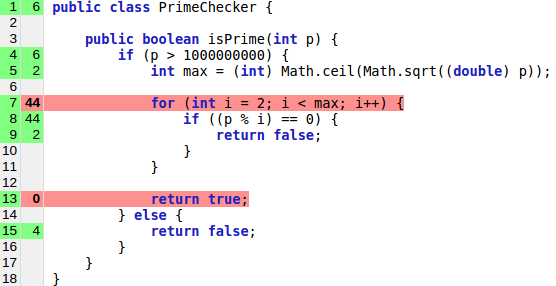
\includegraphics[width=.65\textwidth]{CoverageAnalysis/PrimeChecker.png}
    \caption{Representative of uncovered branches in PrimeChecker.}
    \label{fig:PrimeCheckerAnalysis}
    \vspace{.5cm} 
\end{minipage}
\end{figure}

It seems that part of the code shown in Figure \ref{fig:ColourPickerAnalysis} is not covered because of the influence of a random number.
Test input has no influence on how this random number behaves.
Therefore, EvoSuite cannot generate an input that satisfies the condition to cover that branch. 

\begin{figure}
\centering
\begin{minipage}[c]{\textwidth}
        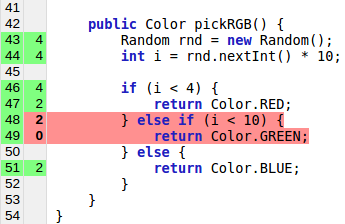
\includegraphics[width=.4\textwidth]{CoverageAnalysis/ColourPicker.png}
    \caption{Representative of uncovered branches in ColourPicker.}
    \label{fig:ColourPickerAnalysis}
    \vspace{.5cm}
\end{minipage}
\end{figure}

In Figure \ref{fig:EnglishNumberToWordsAnalysis}, the \verb|convert(long number)| function accepts a parameter of type \emph{long}.
EvoSuite fails to generate larger numbers to cover the red highlighted lines.
Surprisingly, EvoSuite does not test the boundaries of the long parameter.
Doing so would have resulted in the coverage of at least one of the uncovered branches.

\begin{figure}
\centering
\begin{minipage}[c]{\textwidth}
        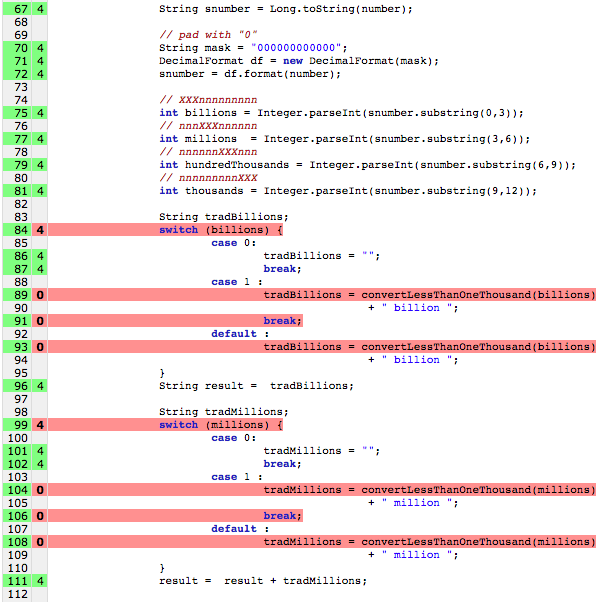
\includegraphics[width=.65\textwidth]{CoverageAnalysis/EnglishNumberToWords.png}
    \caption{Representative of uncovered branches in EnglishNumberToWords.}
    \label{fig:EnglishNumberToWordsAnalysis}
    \vspace{.5cm}
\end{minipage}
\end{figure}


In order to cover the two branches that were not covered by EvoSuite-generated tests in Figure \ref{fig:StringsAnalysis}, a tester would need to input specific strings with a high or low surrogate. 
EvoSuite does not know what high and low surrogate mean and as it does not fall under standard String input, it cannot cover these two branches. 

\begin{figure}
\centering
\begin{minipage}[c]{\textwidth}
        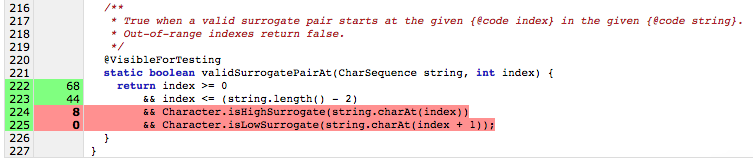
\includegraphics[width=.9\textwidth]{CoverageAnalysis/Strings.png}
    \caption{Representative of uncovered branches in Strings.}
    \label{fig:StringsAnalysis}
    \vspace{.5cm}
\end{minipage}
\end{figure}

In Figure \ref{fig:IntMathAnalysis}, a simple optimization in the case that a left-shift in the power function can be used in not covered.
Since EvoSuite cannot directly reason about the source code, it does not know that such a branch exists and thus there is a possibility that it goes undetected.
This is one of the issues that can arise when using a black-box approach.

\begin{figure}
\centering
\begin{minipage}[c]{\textwidth}
        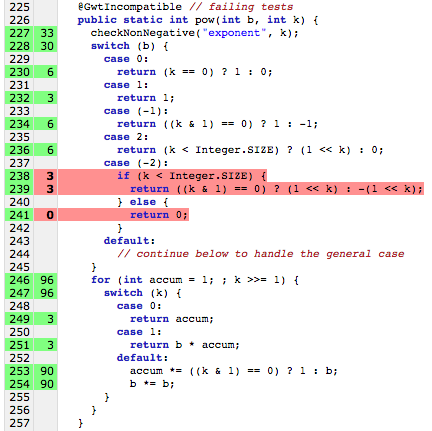
\includegraphics[width=.65\textwidth]{CoverageAnalysis/IntMath.png}
    \caption{Representative of uncovered branches in IntMath.}
    \label{fig:IntMathAnalysis}
    \vspace{.5cm}
\end{minipage}
\end{figure}

\section{Conclusion and Discussions}

EvoSuite is a very promising automated test case generation tool but it encounters some difficulties during the process.
The generated tests can be obscure to read and various branches may remain uncovered.
The main reason found to have unfulfilled goals comes from a lack of knowledge and ability to reason regarding the internal code structure to generate specific input values required to cover a branch.
If there is a condition for which a specific input value is necessary, EvoSuite occasionally does not find the input value to reach that branch.

This is a limitation of any black-box testing tool, which could be improved by analyzing the source code of the system under test.
These improvements would shift the scope of EvoSuite being a black-box testing tool to a more white-box testing tendency.

But a white-box approach does not solve the problems regarding automated test case generation.
The PrimeChecker CUT shows another difficulty, even when applying white-testing techniques to EvoSuite: it requires a significant amount of resources and time to find the required input value to cover a specific branch, e.g. finding a very large prime number.

The experiment for this research performed an exploratory analysis on the correlations between cyclomatic complexity, code coverage and test readability.
Findings indicate that the cyclomatic complexity of the CUT has no apparent influence on the total branch coverage reached.
Additionally, a weak positive correlation of 0.3044 between cyclomatic complexity and readability of the automatically generated tests is found.
Due to the limited size of the dataset used, no definite conclusion can be drawn from these findings.
However, it does indicate that it might be interesting to pursue an in-depth study on a larger scale that will look at the correlation between cyclomatic complexity and the readability of automatically generated tests.
This target of research could have meaningful implication for the design of test oracles after automated test case generation. 

\newpage

\bibliographystyle{plain}
\bibliography{ref.bib}

\newpage

\appendix
\section{Usability of EvoSuite}

In this section, we briefly explore the usability of EvoSuite.
Automated test case generation is a real solution for the burden software testing can be. 
But if a tool like EvoSuite that provides such automation is difficult to use, it does not add much ease to the process of testing. 
We provide with a report on problems encountered when using the tool on Microsoft Windows 10, and on further issues concerning Maven and EvoSuite. 

\subsection{Problems Encountered}

In this part, we report the issues that we encountered during installation and working with automated test generation tool EvoSuite. 
The operating system is Microsoft Windows 10, 64bit. 
After a proper installation, according to the guidelines from the official site \verb|http://www.evosuite.org/| and choosing one of the different ways to execute a test generation tool, namely run EvoSuite from the command line. 
The tool is assembled and compiled in an independent executable jar (e.g., \verb|evosuite.jar|). 
The CUT that we have chosen is Joda-Time that provides API that replaces the standard Java date and time classes. 
However, we discovered a problem on one of the working stations after invoking the given command: 

\verb|$ java -jar evosuite.jar -generateSuite -projectCP <class_path> -class <class_name>|,

where the option \-class is used to define the CUT, and the option -projectCP is used to indicate the classpath.
The error message is shown in figure \ref{fig:error}.

Theoretically, if the correct path is provided, this approach is supposed to work fine if EvoSuite is specified in a "static" context, e.g., when the class path does not change, and a user only changes the CUT's file name.
The installed version of JDK is \verb|1.8.0_60|. 
The system and user variables of the system are defined as follows: \verb|JAVA_HOME| variable is set at \verb|jdk1.8.0_60| and \verb|PATH| at \verb|jdk1.8.0_60/bin|.
However, one of the possible reasons for triggering that error was the assumption that the User Environment variables were not properly set. 
The \verb|PATH| and \verb|JAVA_HOME| variable were excluded from the system variables list but apparently that did not lead to a positive outcome and the possibility to run the test suite to the end. 
Before executing the command that is supposed to generate tests, the following command was executed to make sure the system could refer to the JDK properly: \verb|PATH=%JAVA_HOME%:%PATH%|. 
Unfortunately, that did not change anything and the error message still appeared. 
Bottom line, even though the similar set of system variables that did not result in desired output.

\begin{figure}
\centering
        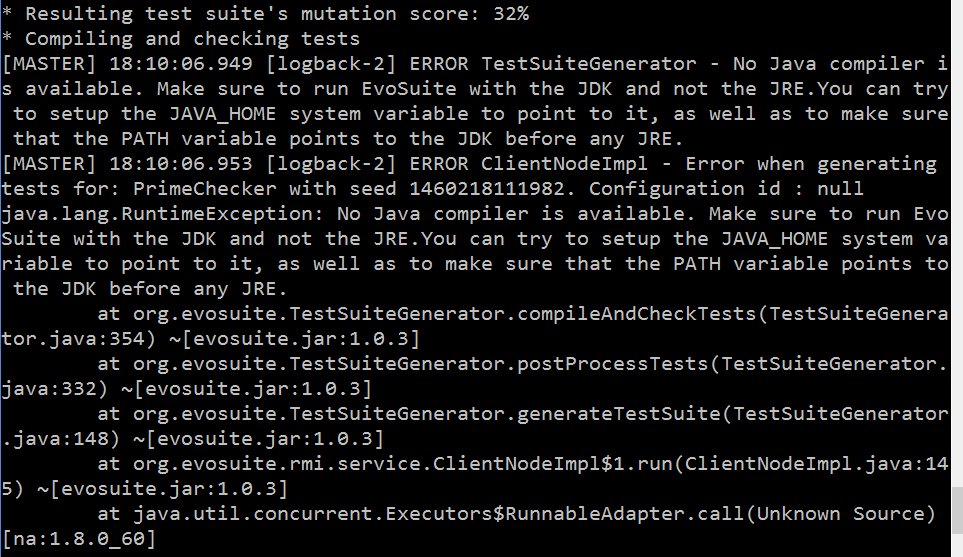
\includegraphics[width=.65\textwidth]{Usability/Error_Evosuite.png}
    \caption{EvoSuite cannot find the Java compiler.}
    \label{fig:error}
    \vspace{.5cm}
\end{figure}

To conclude, a certain set of the environment variables and JDK options did not provide the opportunity for properly set characteristics of the operating system in order to provide the needed scenario to run EvoSuite. 
The absence of detailed documentation and lack of experience resulted in the impossibility of automated test to be generated on the Windows 10 system. 
Nevertheless, when EvoSuite works, it is an effective tool for generating tests to simplify the testing process for developers.
Is a stated solution that will definitely expand its role in the process of automated test generation which will be adopted by software engineers.

\subsection{Maven and EvoSuite}

Generating tests is not all - we need to get these tests to run.
Joda-Time and our own projects made use of Maven as a software project management and comprehension tool. 
Getting EvoSuite dependencies right in the Maven setup is relatively trivial, but it did not work well with other plugins used by the projects.

For example, we integrated Cobertura in each project to calculate branch coverage and cyclomatic complexity. 
Cobertura uses bytecode instrumentation to perform code coverage checks within a class and creates a new class file for the CUT. 
EvoSuite generates tests that are run inside an EvoSuite-dependent sandbox, meaning EvoSuite has its own type of runner. 
When running \verb|mvn corbertura:cobertura| to generate Coberura reports, the tests need to be executed within this sandbox.
The runner attempts to find the CUT but instead runs into two classes: the original CUT, and the class instrumented by Cobertura. 
This confusion causes the JVM to throw a \verb|ClassNotFoundException| and the tests do not get executed. 

To circumvent this problem, it was necessary to manually remove the EvoSuite sandboxing and any EvoSuite dependency within the generated tests. 
Some generated tests used specific EvoSuite assertions to see if an exception was thrown. 
These assertions, unfortunately, had to be removed to generate Cobertura reports. 

\section{Code Snippets}

In this section, we provide code snippets from classes we ran EvoSuite on.

\subsection{PrimeChecker}

\begin{lstlisting}[language=Java, caption=PrimeChecker]
public class PrimeChecker {

    public boolean isPrime(int p) {
        if (p > 1000000000) {
            int max = (int) Math.ceil(Math.sqrt((double) p));

            for (int i = 2; i < max; i++) {
                if ((p % i) == 0) {
                    return false;
                }
            }

            return true;
        } else {
            return false;
        }
    }
}
\end{lstlisting}

\subsection{IntStack}

\begin{lstlisting}[language=Java, caption=IntStack]
public class IntStack {
    private int[] stack;
    private int top_index;

    public IntStack(int capacity) {
        stack = new int[capacity];
        top_index = -1;
    }

    public void push(int i) throws Exception {
        if (!isFull()) {
            int new_top_index = top_index + 1;
            stack[new_top_index] = i;
            top_index = new_top_index;
        } else {
            throw new Exception("Stack is full");
        }
    }

    public int pop() throws Exception {
        if(!isEmpty()) {
            int i = peek();
            top_index = top_index - 1;
            return i;
        } else {
            throw new Exception("Stack is empty");
        }
    }

    public int peek() throws Exception {
        if (!isEmpty()) {
            return stack[top_index];
        } else {
            throw new Exception("Stack is empty");
        }
    }

    public boolean isEmpty() {
        return top_index == -1;
    }

    public boolean isFull() {
        return top_index == capacity() - 1;
    }

    public int capacity() {
        return stack.length;
    }
}
\end{lstlisting}

\subsection{ColourPicker}

\begin{lstlisting}[language=Java, caption=ColourPicker]
public class ColourPicker {

    public Color toColor(boolean number, int i, String name) {
        if (number) {
            if (i == 0) {
                return Color.WHITE;
            } else if (i == 1) {
                return Color.RED;
            } else if (i == 2) {
                return Color.GREEN;
            } else if (i == 3) {
                return Color.BLUE;
            } else if (i == 4) {
                return Color.MAGENTA;
            } else if (i == 5) {
                return Color.YELLOW;
            } else if (i == 6) {
                return Color.CYAN;
            } else {
                return Color.BLACK;
            }
        } else {
            switch (name) {
                case "red" : return Color.RED;
                case "green" : return Color.GREEN;
                case "blue" : return Color.BLUE;
                case "yellow" : return Color.MAGENTA;
                case "magenta" : return Color.YELLOW;
                case "cyan" : return Color.CYAN;
                default : if(i == 0) {
                    return Color.WHITE;
                } else {
                    return Color.BLACK;
                }
            }
        }
    }

    public Color pickRGB() {
        Random rnd = new Random();
        int i = rnd.nextInt() * 10;

        if (i < 4) {
            return Color.RED;
        } else if (i < 7) {
            return Color.GREEN;
        } else {
            return Color.BLUE;
        }
    }
}
\end{lstlisting}

\subsection{EnglishNumberToWords}

Source: \url{http://www.rgagnon.com/javadetails/java-0426.html}.
\begin{lstlisting}[language=Java, caption=EnglishNumberToWords]
public class EnglishNumberToWords {
	private static final String[] tensNames = {
			"",
			" ten",
			" twenty",
			" thirty",
			" forty",
			" fifty",
			" sixty",
			" seventy",
			" eighty",
			" ninety"
	};

	private static final String[] numNames = {
			"",
			" one",
			" two",
			" three",
			" four",
			" five",
			" six",
			" seven",
			" eight",
			" nine",
			" ten",
			" eleven",
			" twelve",
			" thirteen",
			" fourteen",
			" fifteen",
			" sixteen",
			" seventeen",
			" eighteen",
			" nineteen"
	};

	private EnglishNumberToWords() {}

	private static String convertLessThanOneThousand(int number) {
		String soFar;

		if (number % 100 < 20){
			soFar = numNames[number % 100];
			number /= 100;
		}
		else {
			soFar = numNames[number % 10];
			number /= 10;

			soFar = tensNames[number % 10] + soFar;
			number /= 10;
		}
		if (number == 0) return soFar;
		return numNames[number] + " hundred" + soFar;
	}


	public static String convert(long number) {
		// 0 to 999 999 999 999
		if (number == 0) { return "zero"; }

		String snumber = Long.toString(number);

		// pad with "0"
		String mask = "000000000000";
		DecimalFormat df = new DecimalFormat(mask);
		snumber = df.format(number);

		// XXXnnnnnnnnn
		int billions = Integer.parseInt(snumber.substring(0,3));
		// nnnXXXnnnnnn
		int millions  = Integer.parseInt(snumber.substring(3,6));
		// nnnnnnXXXnnn
		int hundredThousands = Integer.parseInt(snumber.substring(6,9));
		// nnnnnnnnnXXX
		int thousands = Integer.parseInt(snumber.substring(9,12));

		String tradBillions;
		switch (billions) {
			case 0:
				tradBillions = "";
				break;
			case 1 :
				tradBillions = convertLessThanOneThousand(billions)
						+ " billion ";
				break;
			default :
				tradBillions = convertLessThanOneThousand(billions)
						+ " billion ";
		}
		String result =  tradBillions;

		String tradMillions;
		switch (millions) {
			case 0:
				tradMillions = "";
				break;
			case 1 :
				tradMillions = convertLessThanOneThousand(millions)
						+ " million ";
				break;
			default :
				tradMillions = convertLessThanOneThousand(millions)
						+ " million ";
		}
		result =  result + tradMillions;

		String tradHundredThousands;
		switch (hundredThousands) {
			case 0:
				tradHundredThousands = "";
				break;
			case 1 :
				tradHundredThousands = "one thousand ";
				break;
			default :
				tradHundredThousands = convertLessThanOneThousand(hundredThousands)
						+ " thousand ";
		}
		result =  result + tradHundredThousands;

		String tradThousand;
		tradThousand = convertLessThanOneThousand(thousands);
		result =  result + tradThousand;

		// remove extra spaces!
		return result.replaceAll("^\\s+", "").replaceAll("\\b\\s{2,}\\b", " ");
	}
}
\end{lstlisting}


\end{document}